\documentclass{article}

\usepackage{geometry}
\usepackage{longtable}
\usepackage[dvipsnames,table]{xcolor}
\usepackage{fancyhdr}
\usepackage{xcolor}
\usepackage[inkscapeformat=png]{svg}
\usepackage{graphicx}
\usepackage{hyperref}
\usepackage{float}
\usepackage{listings}
\usepackage{amssymb}
\usepackage{amsmath}
\usepackage{enumitem}
\usepackage{parskip}

% Choose paper size
\geometry{letterpaper, top=25.4mm, bottom=25.4mm, left=25.4mm, right=25.4mm}

\color{black}
\fancyhf{}
\renewcommand{\headrulewidth}{1pt}
\renewcommand{\footrulewidth}{1pt}

% Define standard IPF color palette
\definecolor{soft-sky-blue}{HTML}{B7DAEB}
\definecolor{orange}{HTML}{FF6633}
\definecolor{cool-grey}{HTML}{91A1B0}
\definecolor{black}{HTML}{000000}
\definecolor{space-blue}{HTML}{003366}
\definecolor{pigeon-blue}{HTML}{5F8396}
\definecolor{sage-green}{HTML}{95A077}
\definecolor{fire-yellow}{HTML}{F9A651}
\definecolor{apple-red}{HTML}{CC4200}
\definecolor{crockadile-green}{HTML}{718944}
\definecolor{slate-grey}{HTML}{607587}
\definecolor{fog-grey}{HTML}{E5E6E9}

% Define certification colors
\definecolor{cert-level-0}{HTML}{CC4200} % apple-red
\definecolor{cert-level-1}{HTML}{FF6633} % orange
\definecolor{cert-level-2}{HTML}{F9A651} % fire-yellow
\definecolor{cert-level-3}{HTML}{B7DAEB} % soft-sky-blue
\definecolor{cert-level-4}{HTML}{5F8396} % pigeon-blue
\definecolor{cert-level-5}{HTML}{718944} % sage-green

\hypersetup{hidelinks}
\pagestyle{fancy}
\pagenumbering{arabic}

\title{
    
\includegraphics[width=8cm] {images/Rocksavage_Tech_RGB_300.png}\vspace{50pt}
    \vspace{10pt} \\
    \textbf{Timer \\
    Product User Guide} \\
    {\small{\textcolor{slate-grey}{rocksavagetech.chiselWare.Timer}}} \\
    \vspace{20pt} IPF certified to level:
    \textbf{\textcolor{cert-level-0}{0} }of 5 \\
    \vspace{5pt}
    
\includegraphics[width=4cm] {images/uncertified.png}
}

\author{Warren Savage}

\fancyhead[L]{Timer Users Guide}
\fancyhead[R]{\leftmark}
\fancyfoot[C]{Rocksavage Technology, Inc.~\copyright~2023}
\fancyfoot[R]{Page \thepage}

\begin{document}

    \maketitle
    \newpage
    \tableofcontents

    \section{Errata and Known Issues}

\subsection{Errata}
None.

\subsection{Known Issues}
None.
    % chktex-file 44
\section{Port Descriptions}

\subsection{Timer/Counter Mode}

The ports for \textbf{Timer/Counter} are shown below in 
Table 1.
 
\renewcommand*{\arraystretch}{1.4}
\begin{longtable}[H]{
  | p{0.20\textwidth}
  | p{0.20\textwidth}
  | p{0.12\textwidth}
  | p{0.43\textwidth} |
  }
  \hline
  \textbf{Port Name} &   
  \textbf{Width} &   
  \textbf{Direction} &   
  \textbf{Description} \\ \hline \hline

  signalOut &       
  1 & 
  Output &       
  Signal generated by timer/counter\\ \hline

  irqOutput &      
  1 & 
  Output &     
  Sent when interrupt is triggered on the Gpio \\ \hline
 
 
  \caption{Timer/Counter Ports Descriptions}\label{table:tc}
\end{longtable}

\subsection{Watchdog Timer Mode}

The ports for \textbf{Watchdog Timer} are shown below in 
Table 1.
 
\renewcommand*{\arraystretch}{1.4}
\begin{longtable}[H]{
  | p{0.20\textwidth}
  | p{0.20\textwidth}
  | p{0.12\textwidth}
  | p{0.43\textwidth} |
  }
  \hline
  \textbf{Port Name} &   
  \textbf{Width} &   
  \textbf{Direction} &   
  \textbf{Description} \\ \hline \hline

  reset &       
  1 & 
  Output &       
  System reset signal\\ \hline

 
  \caption{WDT Ports Descriptions}\label{table:wdt}
\end{longtable}

\subsection{Real Time Clock Mode}

The ports for \textbf{Real Time Clock} are shown below in 
Table 1.
 
\renewcommand*{\arraystretch}{1.4}
\begin{longtable}[H]{
  | p{0.20\textwidth}
  | p{0.20\textwidth}
  | p{0.12\textwidth}
  | p{0.43\textwidth} |
  }
  \hline
  \textbf{Port Name} &   
  \textbf{Width} &   
  \textbf{Direction} &   
  \textbf{Description} \\ \hline \hline

  irqOutput &      
  1 & 
  Output &     
  Sent when interrupt is triggered on the Gpio \\ \hline

 
  \caption{RTC Ports Descriptions}\label{table:rtc}
\end{longtable}

\subsection{APB3 Interface}
The \textbf{APB3 Interface} is a regular APB3 Slave Interface. All signals supported are shown below in 
Table 2. See the \textit{AMBA APB Protocol Specifications} for a complete description of the signals. The width of several ports is controlled 
by the following input parameters:

\begin{itemize}[noitemsep]
  \item \textit{dataWidth} is the width of PWDATA and PRDATA in bits
  \item \textit{addrWidth} is the width of PADDR in bits
\end{itemize}
 
\renewcommand*{\arraystretch}{1.4}
\begin{longtable}[H]{
  | p{0.20\textwidth}
  | p{0.20\textwidth}
  | p{0.12\textwidth}
  | p{0.43\textwidth} |
  }
  \hline
  \textbf{Port Name} &   
  \textbf{Width} &   
  \textbf{Direction} &   
  \textbf{Description} \\ \hline \hline

  PCLK &       
  1 &       
  Input &       
  Positive edge clock \\ \hline

  PRESETN &       
  1 &       
  Input &       
  Active low reset \\ \hline

  PSEL &       
  1 & 
  Input &       
  Indicates slave is selected and a data transfer is required \\ \hline

  PENABLE &        
  1 & 
  Input &       
  Indicates second cycle of APB transfer \\ \hline

  PWRITE &        
  1 & 
  Input &       
  Indicates write access when HIGH and read access when LOW\\ \hline

  PADDR &      
  \textit{addrWidth} & 
  Input &     
  Address bus \\ \hline

  PWDATA &      
  \textit{dataWidth} & 
  Input &     
  Write data bus driven when PWRITE is HIGH\\ \hline

  PRDATA &      
  \textit{dataWidth} & 
  Output &     
  Read data bus driven when PWRITE is LOW\\ \hline
 
  PREADY &        
  1 & 
  Output &       
  Transfer ready \\ \hline

  PSLVERR &        
  1 & 
  Output &       
  Transfer error \\ \hline

  \caption{APB Ports Descriptions}\label{table:interface}
\end{longtable}

    \section{Parameter Descriptions}

The parameters for \textbf{Timer} are shown below in Table~\ref{table:params}.

\renewcommand*{\arraystretch}{1.4}
\begin{longtable}[H]{
    | p{0.25\textwidth}
    | p{0.10\textwidth}
    | p{0.05\textwidth}
    | p{0.05\textwidth}
    | p{0.47\textwidth} |
  }
  \hline
  \textbf{Name} &
  \textbf{Type} &
  \textbf{Min}  &
  \textbf{Max}  &
  \textbf{Description}            \\ \hline \hline

  dataWidth     &
  Int           &
  8             &
  $\ge$ 8       &
  The width of the data bus in bits      \\ \hline

  addressWidth  &
  Int           &
  8             &
  $\ge$ 8       &
  The width of the address bus in bits   \\ \hline

  countWidth    &
  Int           &
  8             &
  $\ge$ 8       &
  The width of the counter in bits       \\ \hline

  prescalerWidth    &
  Int           &
  8             &
  $\ge$ 8       &
  The width of the prescaler in bits       \\ \hline

  \caption{Parameter Descriptions}\label{table:params}
\end{longtable}

The Timer is instantiated into a design as follows:

\begin{lstlisting}[language=Scala]
  // Instantiate Timer with default parameters
  val myTimer = new Timer(TimerParams(
    dataWidth = 32,
    addressWidth = 32,
    countWidth = 64,
    prescalerWidth = 32
  ))
\end{lstlisting}
    \section{Theory of Operations}

\subsection{Introduction}
The \textbf{Timer} is a configurable timer module that supports a variety of timing functions, including PWM generation and interrupt signaling. It features a counter that can be configured with a prescaler, maximum count value, and PWM ceiling value.

\begin{figure}[h]
  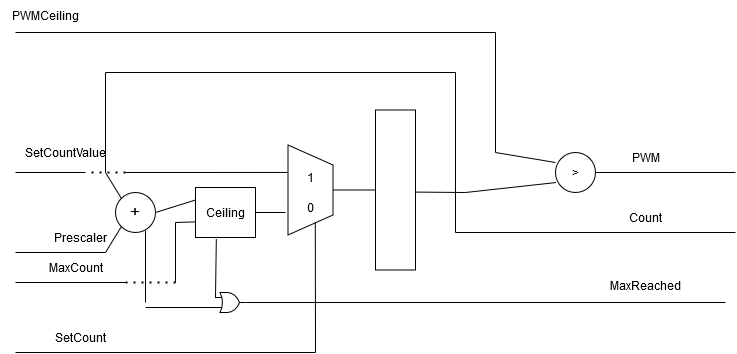
\includegraphics[width=0.80\textwidth]{images/TimerDragram.drawio.png}
  \caption{Timer Diagram}\label{fig:timer-diagram}
\end{figure}

The Timer module provides the following outputs:

\begin{itemize}[noitemsep]
  \item{\textit{count}: Current value of the counter.}
  \item{\textit{maxReached}: Signal indicating the counter has reached its maximum value.}
  \item{\textit{pwm}: PWM output signal with a duty cycle controlled by \textit{pwmCeiling}.}
  \item{\textit{interrupt}: Interrupt signal indicating timer events (e.g., max reached).}
\end{itemize}

\subsection{Interface Timing}
The Timer operates on a synchronous clock and provides outputs that are valid on the rising edge of the clock. The timing diagram below illustrates the behavior of the Timer when the counter reaches its maximum value and generates an interrupt.

% \begin{figure}[h]
%   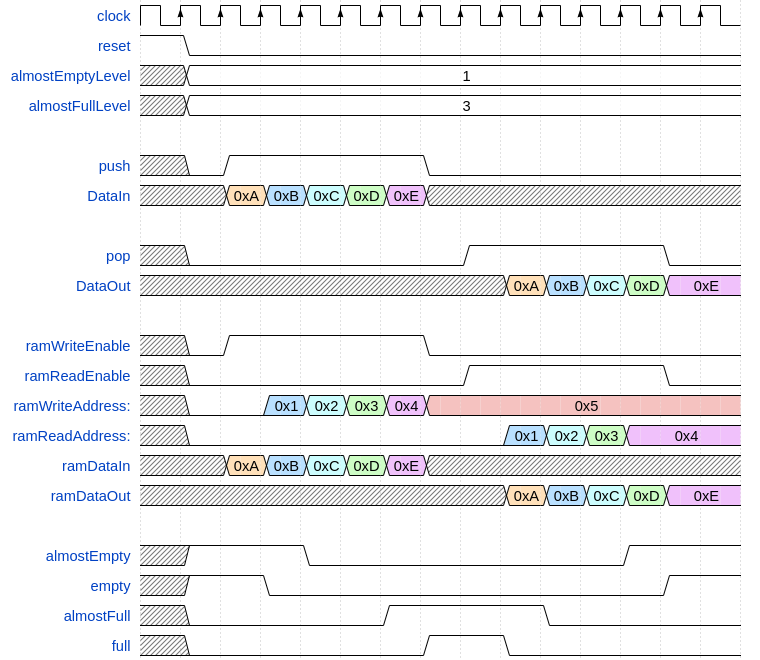
\includegraphics[width=\textwidth]{images/timing.png}
%   \caption{Timing Diagram}\label{fig:timing}
% \end{figure}
    \section{Simulation}

\subsection{Tests}
The test bench generates a number (default is 50) configurations of the
DynamicFifo that are highly randomized. There are two flavors of tests:

\begin{itemize}
  \item {Directed tests that fill the FIFO with random data and then read back
        the results to verify that the read data matches the writted data.}
  \item {Lengthy random tests that are used to check odd combinations of
        configurations and to compile code coverage data.}
\end{itemize}

\subsection{Code coverage}
All inputs and outputs are checked to insure each toggle at least once. An error
will be thrown in case any port fails to toggle.

The only exception are the \emph{almostEmptyLevel} and \emph{almostFullLevel}
which are intended to be static during each simulation. These signals are
excluded from coverage checks.

\subsection{Running simulation}

Simulations can be run directly from the command prompt as follows:

\begin{verbatim}
  $ sbt "test"
\end{verbatim}

or from make as follows:

\texttt{\$ make test}
    \section{Synthesis}

\subsection{Area}
The Timer module has been synthesized in various configurations, and the following results should be representative of what a user should expect in their own technology.

\renewcommand*{\arraystretch}{1.4}
\begin{longtable}[H]{
    | p{0.20\textwidth}
    | p{0.15\textwidth}
    | p{0.15\textwidth}
    | p{0.15\textwidth}
    | p{0.15\textwidth} |
  }
  \hline
  \textbf{Config Name}   &
  \textbf{dataWidth}     &
  \textbf{addressWidth}  &
  \textbf{countWidth}    &
  \textbf{Gates}           \\ \hline \hline

  config1 &
  8 &
  8 &
  8 &
  901 \\ \hline

  config2 &
  16 &
  16 &
  16 &
  1809 \\ \hline

  config3 &
  32 &
  32 &
  32 &
  3591 \\ \hline

  config4 &
  64 &
  64 &
  64 &
  7076 \\ \hline

  \caption{Synthesis results}\label{table:area}
\end{longtable}

\subsection{SDC File}
An \texttt{.sdc} file is generated to provide synthesis and static timing analysis tools guidance for synthesis.

The \texttt{Timer.sdc} file is emitted and found in the \texttt{./syn} directory.

\subsection{Timing}
The following timing was extracted using the generated \texttt{.sdc} files.

\renewcommand*{\arraystretch}{1.4}
\begin{longtable}[H]{
    | p{0.20\textwidth}
    | p{0.08\textwidth}
    | p{0.12\textwidth}
    | p{0.13\textwidth}
    | p{0.15\textwidth}
    | p{0.15\textwidth} |
  }
  \hline
  \textbf{Config Name}   &
  \textbf{Period}        &
  \textbf{Duty Cycle}    &
  \textbf{Input Delay}   &
  \textbf{Output Delay}  &
  \textbf{Slack}           \\ \hline \hline

  config1 &
  5ns &
  50\% &
  20\% &
  20\% &
  2.93 (MET) \\ \hline

  config2 &
  5ns &
  50\% &
  20\% &
  20\% &
  2.69 (MET) \\ \hline

  config3 &
  5ns &
  50\% &
  20\% &
  20\% &
  2.80 (MET) \\ \hline

  config4 &
  5ns &
  50\% &
  20\% &
  20\% &
  2.77 (MET) \\ \hline

  \caption{Static Timing Analysis results}\label{table:timing}
\end{longtable}

\subsection{Multicycle Paths}
None.

\end{document}